\documentclass[a4paper,12pt]{article}

\usepackage[justification=centering, margin=2cm, labelfont=bf, font={small}]{caption}
\usepackage{float}
\usepackage{subcaption}
\usepackage{graphicx}


\setlength{\parskip}{1em}
\setlength{\parindent}{0em}
\title{Article Review}
\author{Jacob Josiah Webber}
\date{March 2017}
 
\begin{document}
\maketitle

\section{Introduction}
This report reviews the article ``Probabilistic Grammars for Music'' \cite{Bod_probabilisticgrammars} by Rens Bod. The article describes the application of probabilistic parsing techniques that were originally developed for natural language processing (NLP). These techniques are used to predict where musical phrases will begin and end when given a melody line. They are trained and tested for accuracy using the Essen Folksong Collection.

This report will summarise the article in question as well as offering a critical review of the claims made. In particular, attention is given to how the parsing techniques proposed might be used generate new music.

\section{Musical Phrases}
When given a melodic line, those with musical training will naturally divide this line up into phrases. In the realm of Western Art music this phrasing is not typically notated, unlike other melodic information such as note pitches and durations. Music of this style is not simply divided into one phrase at a time, often there is a hierarchy of phrasing. For example in the Classical period, music was typically divided into balanced phrase pairs. Figure \ref{haydn} gives a particularly paradigmatic example from this period as annotated in \cite{music-theory}. This example has limited ambiguity. While it could be argued that what is described in \cite{music-theory} as a ``phrase member'' deserves full recognition as a phrase in itself, this is more just a question of terminology, and most would agree with the general hierarchy presented.

\begin{figure}
\centering
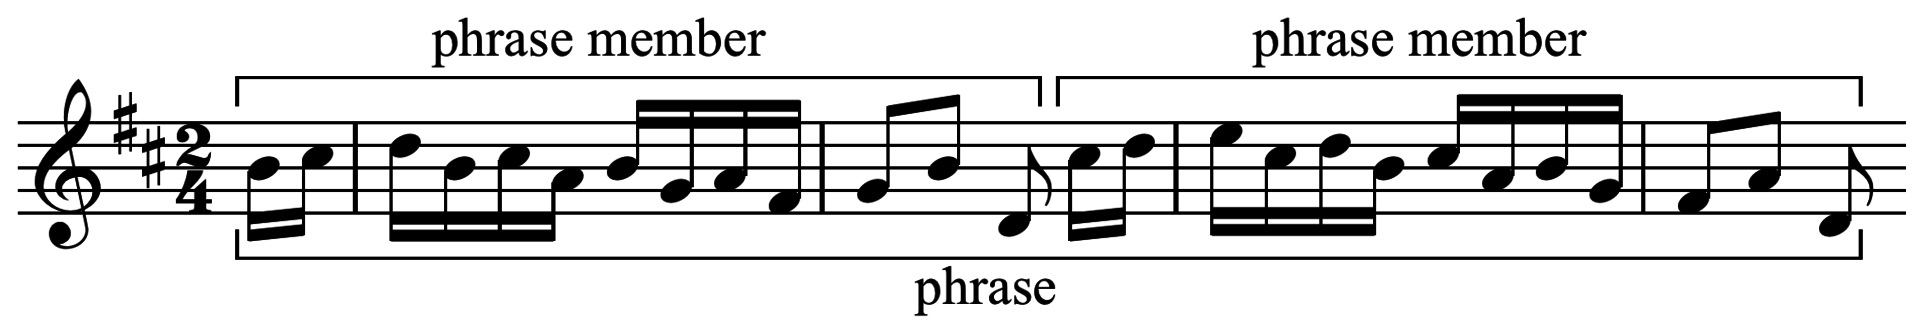
\includegraphics[width=\textwidth]{diagrams/Haydn}
\caption{Example of balanced phrase pair from  Haydn's Trio no. 1 in G Major}
\label{haydn}
\end{figure}

The clarity of the structure in music of this era means that musicologists often depend on this style to describe phrasing. This is so in \cite{Bod_probabilisticgrammars}, where Mozart's famous G Minor Symphony is used for this purpose.

%other styles are not so simple. Music from the romantic era is characterised by long flowing phrases that are much more ambiguous.


%Nevertheless, while there is always some ambiguity, the majority of interpretations of phrase start and end points will be relatively uncontroversial.

\section{The Essen Folksong Collection}
\label{essensec}

While music from the classical era is used to describe phrasing to the reader, the actual examples that make up the corpus used for experiment come from the Essen Folksong Collection. This is a large corpus of European folksongs notated using the Essen Associative Code (ESAC). This provides a way of notating music using standard characters, which is therefore easy for computers to store and process. For a detailed description of how this notation works readers should see \cite{Bod_probabilisticgrammars}.

The Collection itself includes 6,251 folk melodies collected under the supervision of Helmut Schaffrath at The University of Essen \cite{essen}. Unlike standard Western musical notation, these melodies have phrasing stored along with the other melodic data. The fact that this data is encoded on such a large corpus gives the opportunity to train and test phrase prediction algorithms. Along with standard practice on the treatment of corpora in NLP, the Essen collection is divided randomly into training and test sets of ratio 5,251:1,000 respectively.  

For the purpose of testing these algorithms, it is necessary to have a system of scoring any generated solution. To do this, a methodology was borrowed from the field of NLP, as proposed in \cite{nlp-score}. This uses the twin notions of \emph{precision} and \emph{recall} defined as:
$$precision = \frac{\#\ correct\ phrases\ in\ P}{\#\ phrases\ in\ P} $$
and
$$recall = \frac{\#\ correct\ phrases\ in\ P}{\#\ phrases\ in\ T} $$
where $P$ is a proposed parse and $T$ is the test set parse from the corpus. Another concept from the field of NLP is used to combine these - that of the F-score. This is given in \cite{manning} as

$$ F\-score = \frac{2 \cdot precision \cdot recall}{precision+recall}. $$

Now that there is a corpus, complete with training and test sets, and a scoring algorithm, it is possible to unleash machine learning techniques devised for NLP on this problem.

\section{Parsing Techniques}

The paper provides results from 3 parsing techniques. The first and least successful of these is the Treebank grammar technique first proposed in \cite{Bod93}. This is an extremely simple context-free technique that stores all structures in the training set and derives a probability based on the frequency of these structures within the training set.

This technique yields a precision of 68.7\%, a recall of 3.4\%, and an F-score of 6.5\% according to the definitions of these measures set out in \ref{essensec}.

The relative nature of these scores is explained by the conservative nature of this parsing technique. The grammar will only output a phrase when a string is provided that exactly matches a phrase in the training set. This means that of those phrases predicted by the parse a high proportion are indeed phrases (68.7\%), but many phrases that do exist are ignored, yielding a very low score for recall and therefore a low F-score. The precision score would be higher if some contextual features where used in parsing, for example so that a common short phrase from the test set would not be predicted in a piece that otherwise has much longer phrases. The recall would be higher if there was some mechanism for predicting phrases that do not exactly exist within the test set.

The next proposed technique, a Markov grammar, addresses some of the conservativity of the Treebank method. This method is applied to NLP in \cite{Seneff1992}. This creates Markov chains at the note level in order to predict the likeliness of a phrase ending given the previous $n$ notes, where $n$ is the order of Markov process. In this case a third-order Markov process was used and produced a  precision of 63.1\%, a recall of 80.2\%, and an F-score of 70.6\%. While the precision in this case is slightly lower than that of the Treebank technique, as would be expected with a more permissive system, the recall is very much higher.

The third technique can be thought of as an extension to the Markov grammar described previously. This uses the Data-Oriented Parsing (DOP) technique to take into account a global context. This context allows factors such as average phrase length in the piece being parsed to be taken into account. As expected, this extra information improves all measured scores. The DOP-Markov parser obtained a precision of 76.6\%, a recall of 85.9\%, and an F-score of 81.0\%. 

Table \ref{resulttab} shows all of these results in full. The results can be summarised by comparing how much information these parsers take into account from their training. The Treebank only operates at the object level, and therefore only remembers familiar objects from the training set. The Markov technique takes into account probabilistically the relation between notes, or sub-object elements and therefore gives better results, although some precision is sacrificed as this yields a less conservative grammar. The final and most successful technique adds to this a global context. It is demonstrated in these cases, therefore, that the more probabilistic data gathered from the training set, the more accurate the phrase predictions will be.

\begin{table}
\centering
\begin{tabular}{ |c|c|c|c| } 
 \hline
 Parsing technique & precision & recall & F-score \\ 
 \hline
 Treebank & 68.7\% & 3.4\% & 6.5\% \\ 
 Markov Grammar & 63.1\% & 80.2\% & 70.6\% \\ 
 Markov + DOP & 76.6\% & 85.9\% & 81.0\% \\ 

 \hline
\end{tabular}
\caption{Table showing full results from the parsing experiments. The Markov and DOP technique was the most successful.}
\label{resulttab}
\end{table}

\section{Other Parsing Techniques}



\section{Critical Review}

\section{Conclusion}

\bibliography{bibliography}
\bibliographystyle{ieeetr}

\end{document}